\begin{center}
	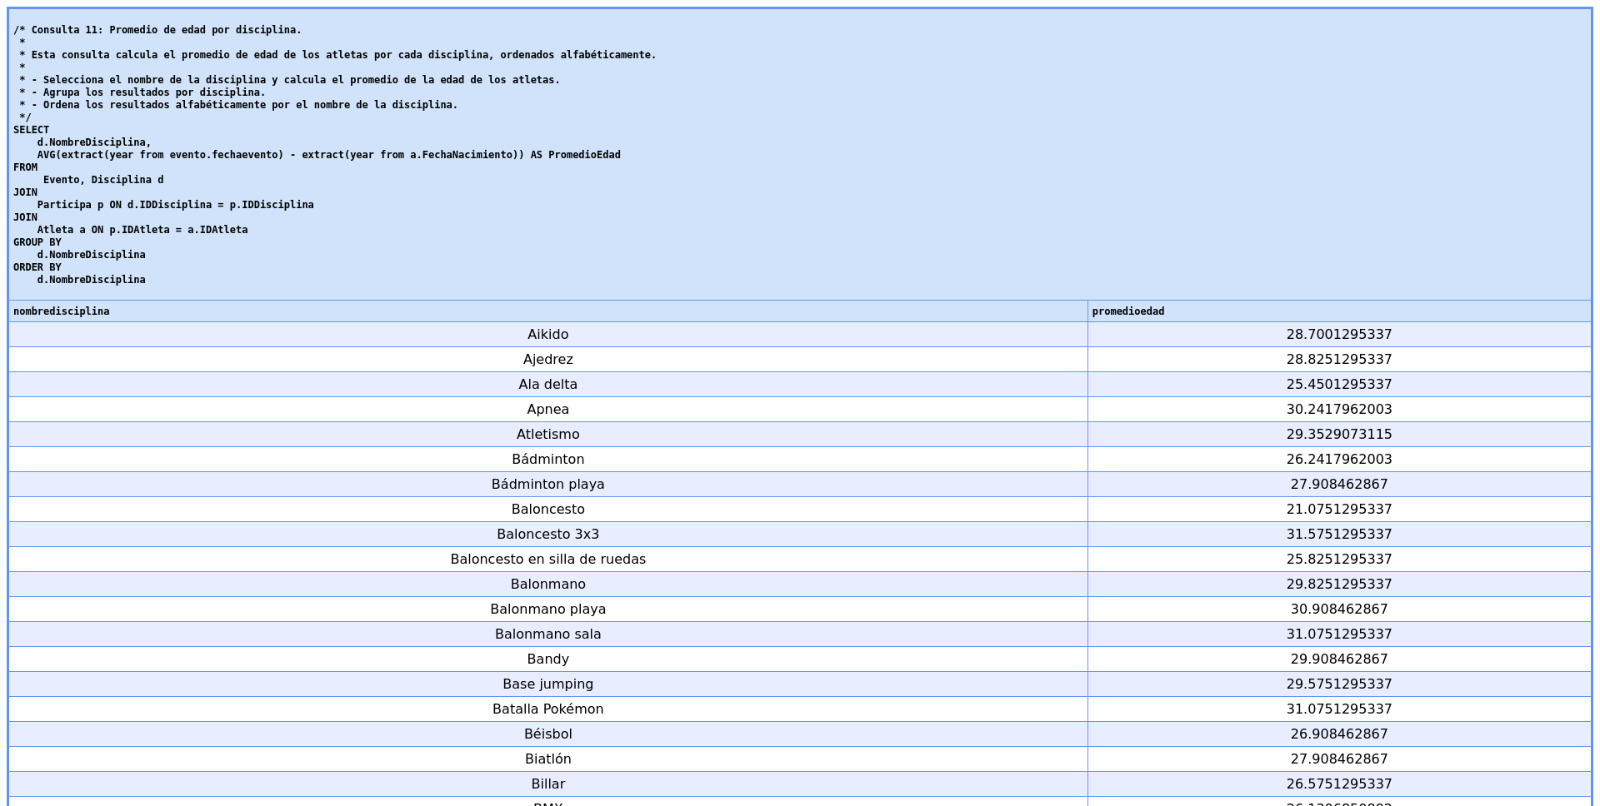
\includegraphics[width=16.5cm]{resources/Chapters/Consultas/Imagenes/Consulta11.jpg} 
	
	Consulta 11. Promedio de edad por disciplina.
\end{center}

\textbf{Propósito de la consulta}

La consulta tiene como objetivo calcular el promedio de edad de los atletas por cada disciplina deportiva. Los resultados están ordenados alfabéticamente por el nombre de la disciplina para facilitar su interpretación.

\textbf{Desglose de la consulta}

\begin{itemize} \item \textbf{Selección de columnas (\texttt{SELECT}):} \begin{itemize} \item \texttt{d.NombreDisciplina}: El nombre de la disciplina, que identifica de forma única cada deporte o actividad. \item \texttt{AVG(EXTRACT(YEAR FROM evento.FechaEvento) - EXTRACT(YEAR FROM a.FechaNacimiento)) AS PromedioEdad}: Calcula el promedio de la diferencia de años entre la fecha del evento y la fecha de nacimiento de los atletas, representando el promedio de edad para cada disciplina. \end{itemize}
	
	\item \textbf{Tablas involucradas (\texttt{FROM} y \texttt{JOIN}):} \begin{itemize} \item \texttt{Evento}: Tabla que contiene información sobre los eventos, incluida la fecha en que se llevaron a cabo. \item \texttt{Disciplina (d)}: Tabla que registra las disciplinas deportivas disponibles. \item \texttt{Participa (p)}: Relaciona a los atletas con las disciplinas en las que participan. \item \texttt{Atleta (a)}: Tabla que almacena información sobre los atletas, incluida su fecha de nacimiento. \item \textbf{Uniones (\texttt{JOIN})}: \begin{itemize} \item Se realiza un \texttt{JOIN} entre \texttt{Disciplina (d)} y \texttt{Participa (p)} usando la clave \texttt{d.IDDisciplina = p.IDDisciplina}. \item Posteriormente, se une \texttt{Atleta (a)} con \texttt{Participa (p)} usando \texttt{p.IDAtleta = a.IDAtleta}. \end{itemize} \end{itemize}
	
	\item \textbf{Agrupación de resultados (\texttt{GROUP BY}):} \begin{itemize} \item La agrupación se realiza por \texttt{d.NombreDisciplina}, lo que permite calcular el promedio de edad de los atletas de forma independiente para cada disciplina. \end{itemize}
	
	\item \textbf{Ordenamiento de resultados (\texttt{ORDER BY}):} \begin{itemize} \item Los resultados se ordenan alfabéticamente por el nombre de la disciplina (\texttt{d.NombreDisciplina}), facilitando su organización y lectura. \end{itemize} \end{itemize}

\textbf{Análisis detallado}

\begin{itemize} \item \textbf{Relación entre tablas:} \begin{itemize} \item La consulta utiliza varias tablas relacionadas: \begin{itemize} \item La tabla \texttt{Disciplina (d)} se conecta con \texttt{Participa (p)} para identificar las disciplinas en las que participan los atletas. \item La tabla \texttt{Atleta (a)} proporciona la información de la fecha de nacimiento de cada atleta, necesaria para calcular su edad. \end{itemize} \item La tabla \texttt{Evento} se utiliza para calcular la edad de los atletas en el año en que ocurrió el evento. \end{itemize}
	
	\item \textbf{Cálculo del promedio de edad:} \begin{itemize} \item La función \texttt{AVG()} calcula el promedio de la diferencia entre: \begin{itemize} \item El año del evento (\texttt{EXTRACT(YEAR FROM evento.FechaEvento)}). \item El año de nacimiento del atleta (\texttt{EXTRACT(YEAR FROM a.FechaNacimiento)}). \end{itemize} \item Esto representa el promedio de edad de los atletas para cada disciplina en el año del evento. \end{itemize}
	
	\item \textbf{Ordenamiento alfabético:} \begin{itemize} \item Ordenar los resultados por \texttt{d.NombreDisciplina} garantiza que las disciplinas estén organizadas de forma alfabética, mejorando la presentación de los datos. \end{itemize} \end{itemize}

\textbf{Posibles escenarios y consideraciones}

\begin{itemize} \item \textbf{Disciplinas sin participación:} \begin{itemize} \item Si una disciplina no tiene atletas registrados en \texttt{Participa}, no aparecerá en los resultados debido al uso de \texttt{JOIN}, lo que implica que solo se consideran disciplinas con participantes. \end{itemize}
	
	\item \textbf{Edad promedio en decimal:} \begin{itemize} \item Los resultados del promedio de edad pueden incluir decimales, lo que representa una aproximación más precisa. \end{itemize}
	
	\item \textbf{Datos de fechas:} \begin{itemize} \item Es importante que las fechas (\texttt{evento.FechaEvento} y \texttt{a.FechaNacimiento}) estén correctamente registradas para evitar errores en el cálculo de la edad. \end{itemize} \end{itemize}

La consulta está diseñada para calcular de manera eficiente el promedio de edad de los atletas por disciplina, proporcionando información valiosa para análisis demográficos y de participación en los eventos deportivos.